\normaltrue
\correctiontrue

%\UPSTIidClasse{11} % 11 sup, 12 spé
%\newcommand{\UPSTIidClasse}{11}

\exer{Mouvement RT  $\star$ \label{C1:05:06:PFD}}
\setcounter{question}{0}\UPSTIcompetence[2]{B2-14}
\UPSTIcompetence[2]{C1-05}
\index{Compétence B2-14}
\index{Compétence C1-05}
\index{Principe fondamental de la dynamique}
\index{PFD}
\index{Mécanisme à 1 translation et 1 rotation}
\ifcorrection
\else
\marginnote{\textbf{Pas de corrigé pour cet exercice.}}
\fi

\ifprof
\else
Soit le mécanisme suivant. On a $\vect{AB}=\lambda(t)\vect{i_0}$ et $\vect{BC}=R\vect{i_2}$ avec $R=\SI{30}{mm}$.
De plus :
\begin{itemize}
\item $G_1=B$ désigne le centre d'inertie de \textbf{1}, on note $m_1$ la masse de \textbf{1};% et $\inertie{G_1}{1}=\matinertie{A_1}{B_1}{C_1}{0}{0}{0}{\bas{1}}$; 
\item $G_2=C$ désigne le centre d'inertie de \textbf{2}, on note $m_2$ la masse de \textbf{2}.% et $\inertie{G_2}{2}=\matinertie{A_2}{B_2}{C_2}{0}{0}{0}{\bas{2}}$.
\end{itemize}

Un vérin électrique positionné entre \textbf{0} et \textbf{1}  permet d'actionner le solide \textbf{1}.
Un moteur électrique positionné entre \textbf{1} et \textbf{2}  permet d'actionner le solide \textbf{2}.

L'accélération de la pesanteur est donnée par $\vect{g}=-g\vect{j_0}$.

\begin{center}
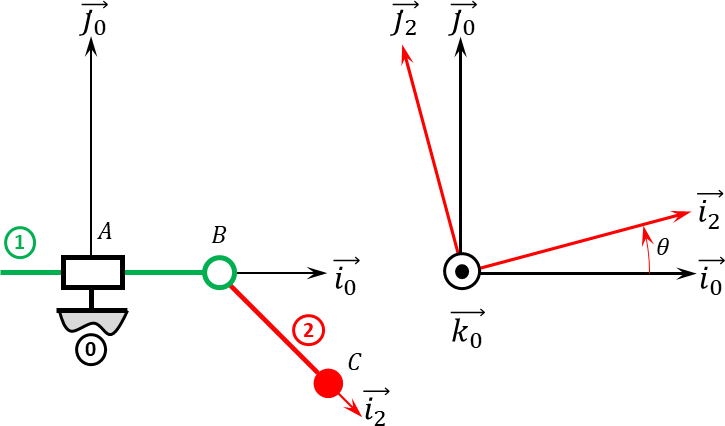
\includegraphics[width=\linewidth]{06_TR_01}
\end{center}
\fi

\question{Réaliser le graphe d'analyse en faisant apparaître l'ensemble des actions mécaniques.}
\ifprof
\begin{center}
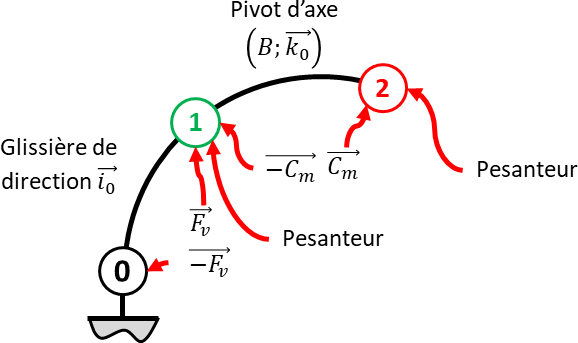
\includegraphics[width=.5\linewidth]{06_TR_02_Cor}
\end{center}
\else
\fi

\question{Proposer une démarche permettant de déterminer les loi de mouvement de \textbf{1} et de \textbf{2} par rapport à $\rep{0}$.}
\ifprof
Ce mécanisme présente deux degrés de liberté indépendants : $\lambda(t)$ et $\theta(t)$. Il est donc nécessaire d'écrire, dans le meilleur des cas, deux équations :
\begin{itemize}
\item une équation traduisant la mobilité de 2 par rapport à 1, soit TMD appliqué à 2 en $B$ en projection sur $\vk{0}$;
\item une équation traduisant la mobilité de 2+1 par rapport à 0, soit TRD appliqué à 1+2 en projection sur $\vi{0}$.
\end{itemize}

\vspace{.5cm}

\begin{itemize}
\item \textbf{On isole 2.}
\end{itemize}

\begin{minipage}[c]{.6\linewidth}
\begin{itemize}
\item \textbf{BAME :}
\begin{itemize}
\item actions de la liaison pivot $\torseurstat{T}{1}{2}$;
\item action du moteur $\torseurstat{T}{\text{mot}}{2}$;
\item action de la pesanteur $\torseurstat{T}{\text{pes}}{2}$.
\end{itemize}
\end{itemize}
\end{minipage} \hfil
\begin{minipage}[c]{.35\linewidth}
\begin{center}
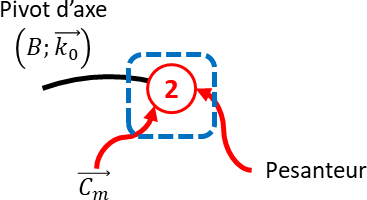
\includegraphics[width=.8\linewidth]{06_TR_03_Cor}
\end{center}
\end{minipage}

\begin{itemize}
\item \textbf{Théorème :} on applique le théorème du moment dynamique en $B$ au solide \textbf{2} en projection sur $\vk{0}$ : $C_{\text{mot}}+\vectm{B}{\text{pes}}{2}\cdot \vk{0}  = \vectmd{B}{2}{0}\cdot \vk{0}$.
\item \textbf{Calcul de la composante dynamique :} considérons le cas où la matrice d'inertie est donnée en $C$. On a donc 
$\vectmd{C}{2}{0}= \deriv{\vectmc{C}{2}{0}}{\rep{0}}=\deriv{\inertie{C}{2}\vecto{2}{0}}{\rep{0}}$. De plus, 
$\babard{B}{C}{2}{0}$ et $\vectrd{2}{0}=m_2 \vectg{C}{2}{0}$.
\end{itemize}

\vspace{.5cm}

\begin{itemize}
\item \textbf{On isole 1+2.}
\end{itemize}

\begin{minipage}[c]{.6\linewidth}
\begin{itemize}
\item \textbf{BAME :}
\begin{itemize}
\item actions de la liaison glissière $\torseurstat{T}{0}{1}$;
\item action de la pesanteur $\torseurstat{T}{\text{pes}}{1}$;
\item action de la pesanteur $\torseurstat{T}{\text{pes}}{2}$;
\item action du vérin $\torseurstat{T}{\text{ver}}{1}$;.
\end{itemize}
\end{itemize}
\end{minipage} \hfil
\begin{minipage}[c]{.35\linewidth}
\begin{center}
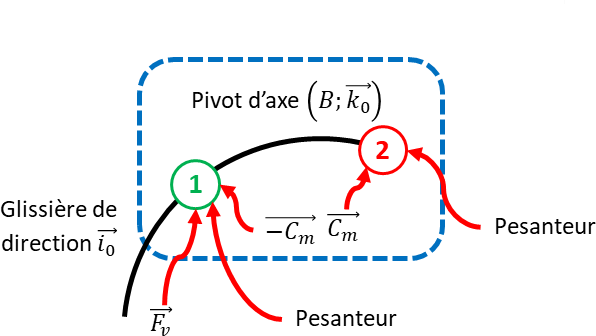
\includegraphics[width=\linewidth]{06_TR_04_Cor}
\end{center}
\end{minipage}

\begin{itemize}
\item \textbf{Théorème :} on applique le théorème de la résultante dynamique à l'ensemble \textbf{1+2} en projection sur 
$\vi{0}$ : 
$\vectf{\text{ver}}{1}\cdot \vi{0}  = \vectrd{1+2}{0}\cdot \vi{0}$.
\item \textbf{Calcul de la composante dynamique :} 
$\vectrd{1+2}{0} = \vectrd{1}{0} +\vectrd{2}{0}$  $= m_1\vectg{G_1}{1}{0} +m_2 \vectg{G_2}{2}{0}$.
\end{itemize}
\else
\fi

\ifprof
\else
\begin{flushright}
\footnotesize{Corrigé  voir \ref{C1:05:06:PFD}.}
\end{flushright}%
\fi